%------------------------------------------------------------------------------------------------------------------------------------------
% Analyza prostredku
%------------------------------------------------------------------------------------------------------------------------------------------
\chapter{ANALYTICKÁ ČÁST} \label{analyza}
\par Před samotným vývojem platformy pro definici a zpracování dat musíme provést průzkum aktuálních technologií zaměřujících se na vývoj webových aplikací a jejich výběr. Výběr technologií, které nám pomohou při vývoji je velice podstatný, protože nám urychlí dodání a co je důležitější, pozdější úprava bude značně jednodušší pokud zvolíme technologie, které nám takovýto pozdější vývoj usnadní.

\par Nejenom vývojovými technologiemi je potřeba se zabývat, ale také aktuálním stavem trhu a toho co uživatelé nejčastěji používají. Proto se v této části zaměříme také průzkumem trhu.

\section{Webové technologie}
\par Aktuální trend v používání webových prohlížečů můžeme vidět na grafu \ref{browser-share}, kde jde jasně vidět že moderní prohlížeče v podání Chrome a Firefox převládají nad tolika vývojáři proklínaný a čím dál tím méně používaný Internet Explorer. dále si uživatelé již uvědomují, že aktualizace prohlížeče je pro zachování zabezpečení nutností a tak naštěstí webové prohlížeče pomalu začínají pořádně fungovat s novým standardem Javascriptu nazvaný EcmaSript 6 (známý též pod názvem ES2015 a ES6). \cite{es6}

\par Nový standard ES6 přináší mnoho vylepšení a mnoho optimalizací. Nicméně ani většina moderních prohlížečů nepodporuje 100 \% tento standard, například prohlížeč \textbf{Google chrome} ve verzi 57 podporuje 97 \% nového standardu, obdobně je na tom \textbf{Edge} (verze 15 podporuje 95 \%) a \textbf{Firefox} (verze 52 zvládá 94\%). \cite{es6-coverage}

\subsection{Webový aplikační rámec}
\par V aktuální době se mnoha vývojářům webových aplikací ověřili takzvané webové aplikační rámce. Dříve hojně využívána knihovna \textbf{jQuery} má již mnoho nástupců jak v podobě knihoven, tak aplikačních rámců. Výhoda takových aplikačních rámců je že se stará v podstatě o veškerou těžkou a neustále se opakující práci a nechává programátorovi volnou ruku při realizaci samostatné aplikace. \cite{framework}

\par V předešlém odstavci bylo použito obou pojmů, jak Javascriptové knihovny, tak aplikačního webového rámce. Tyto pojmy dost často vedou k hádkám a nedorozumění, kdy valná většina programátorů nerozumí rozdílům mezi aplikačním rámcem a knihovnou.
\begin{itemize}
\item \textbf{Javascriptová knihovna} slouží ke konání jednoho úkolu. Vezměme si například výrobu kávy, můžeme si postavit vodu na oheň ohřát ji, rozemlít zrnka kávy a tento prášek zalít horkou vodou. Každý jeden nástroj by představoval knihovnu.
\item \textbf{Aplikační webový rámec} má na starosti veškerou práci a často zahrnuje přesně definovanou architekturu. Pokud si vezmeme příklad s kávou, aplikační webový rámec by byl kávovar, do kterého nalijeme vodu a nasypeme kávová zrna. \cite{framework-vs-library}
\end{itemize}

\paragraph{Angular.js} je plnohodnotný aplikační rámec, v aktuální době pravděpodobně nejpoužívanější. \footnote{Přesná čísla se určit nedají, nicméně více informací o popularitě se můžete dočíst zde: \url{https://hackernoon.com/5-best-javascript-frameworks-in-2017-7a63b3870282\#.ufk9gznfd}}.

\par Strukturální webový aplikační rámec, pro dynamické webové aplikace. Jeho přední výhodou je že se soustřeďuje na tvoření jednostránkových aplikací. Takže často snižuje počet dat nutných pro načtení a pracování s aplikací. První datum vydaní bylo v roce 2010 a v roce 2016 byla vydána verze 2, která umožňuje vytvářet uživatelské rozhraní jak pro webové, tak pro mobilní aplikace.\cite{angular-js}

\paragraph{React.js} není plnohodnotný aplikační rámec, jako \textbf{Angular.js}, nicméně je velkým hráčem na poli vývoje webových aplikací. Jeho výhodou je jeho jednoduchost, nastavení aplikace a počáteční vývoj je velice jednoduchý, nicméně nedokáže tolik věcí co plnohodnotný rámec. Samostatný ovšem není příliš vhodný, potřebuje několik rozšíření, které z něho udělají silnějšího hráče, to ale vede k jeho zkomplikování  a častým problémům s nastavením. \cite{react-js}

\paragraph{Vue.js} je progresivní rámec, pro vytváření uživatelských rozhraní. Jeho tvůrci kladli důraz na jeho jednoduchost použití a inspirovali se v \textbf{React.js}, výhodou oproti zmíněnému má použití s webovou stránkou, kdy se nesnaží obcházet její vykreslování, ale pracuje přímo s html elementy. Dále je tento rámec také zaměřen na práci s jednostránkovou aplikací, takže je výborným kompromisem mezi \textbf{Angular.js} -- který může být příliš náročný pro pochopení, a \textbf{React.js} -- který může vést ke zkomplikování při použití s více rozšířeními. \cite{vue-js}

\subsection{Silné vs. slabé typování}
\par Pro vývoj responzivních webových aplikací se používá Javascript, který je ale slabě typovaný. To znamená že proměnná nemá předem určený pevný typ a může ho během chodu aplikace měnit. To může mít za následek chyby spojené s očekávaným typem, který může být chybný. Takže například při očekávání čísla budeme sčítat, ale aplikace nám během jejího chodu vrátila text. Takový problém může vést až k pádu, případně zamrznutí aplikace. Proto vznikl způsob jak přivést silné typování do slabě typovaných jazyků, jejich zástupci jsou \textbf{Typescript} a \textbf{Flow}.

\paragraph{Typescript} je podmnožinou Javascriptu, to znamená že veškeré soubory jsou přeloženy do předem vybrané verze specifikace a ty jsou poté spuštěny v prohlížeči. Není tedy nutné nutit uživatele do používání jiného prohlížeče. Velkou výhodou je také to, že se tým okolo Typescriptu snaží co nejvíce sledovat trend vývoje Javascriptu a tak přináší mnoho novinek ještě před tím, než je začnou používat prohlížeče. Takže je možné použít velkou část nových technologií, bez nutnosti psát ne zrovna příjemně čitelný kód. \cite{typescript}

\paragraph{Flow} je další způsob jak přivést silné typování do světa Javascriptu, oproti \textbf{Typescriptu} má výhody, že problémy s implicitní deklarací, které mohou nastat během používání aplikace jsou lépe vyhodnoceny a programátor je o tomto informován již během překladu aplikace. Ale jeho nevýhodou je, že nesleduje takovou měrou nejnovější trendy a je často pozadu. Někdy schválně, protože pro překlad novějších definic do staršího použití existují další nástroje. \cite{flow}

\subsection{Responzivní aplikační rámec}
\par Pro usnadnění používání webových aplikací na jakémkoliv zařízení vzniká aktuálně mnoho knihoven a aplikačních rámců, které mají za úkol sjednotit design napříč několika aplikacemi a také jejich responzibilitu. To znamená že stejná aplikace se bude chovat a vypadat stejně bez ohledu na to, na jakém zařízení ji otevřeme (mobilní zařízení, tablet, počítač, televize, atd.)

\paragraph{Material design} vznikl na popud zjednodušení a zpřehlednění uživatelského rozhraní, jeho hlavním zaměřením je dotek, hlas a kliknutí. Definuje tři pravidla \textbf{Material je metafora} -- chytře využívat prostor a pohyb jednotlivých elementů. \textbf{Tučné, grafické, záměrné} -- základními stavebními bloky jsou typografie, mřížka, místo, barva a použití obrázků. \textbf{Pohyb má význam} -- pokud uživatel vykoná nějakou akci design mu napoví jaká akce se stane pohybem. \cite{material} Příklad aplikace napsané pomocí Materialu můžeme vidět na \ref{material-fig}.

\begin{figure}[htp]
\centering
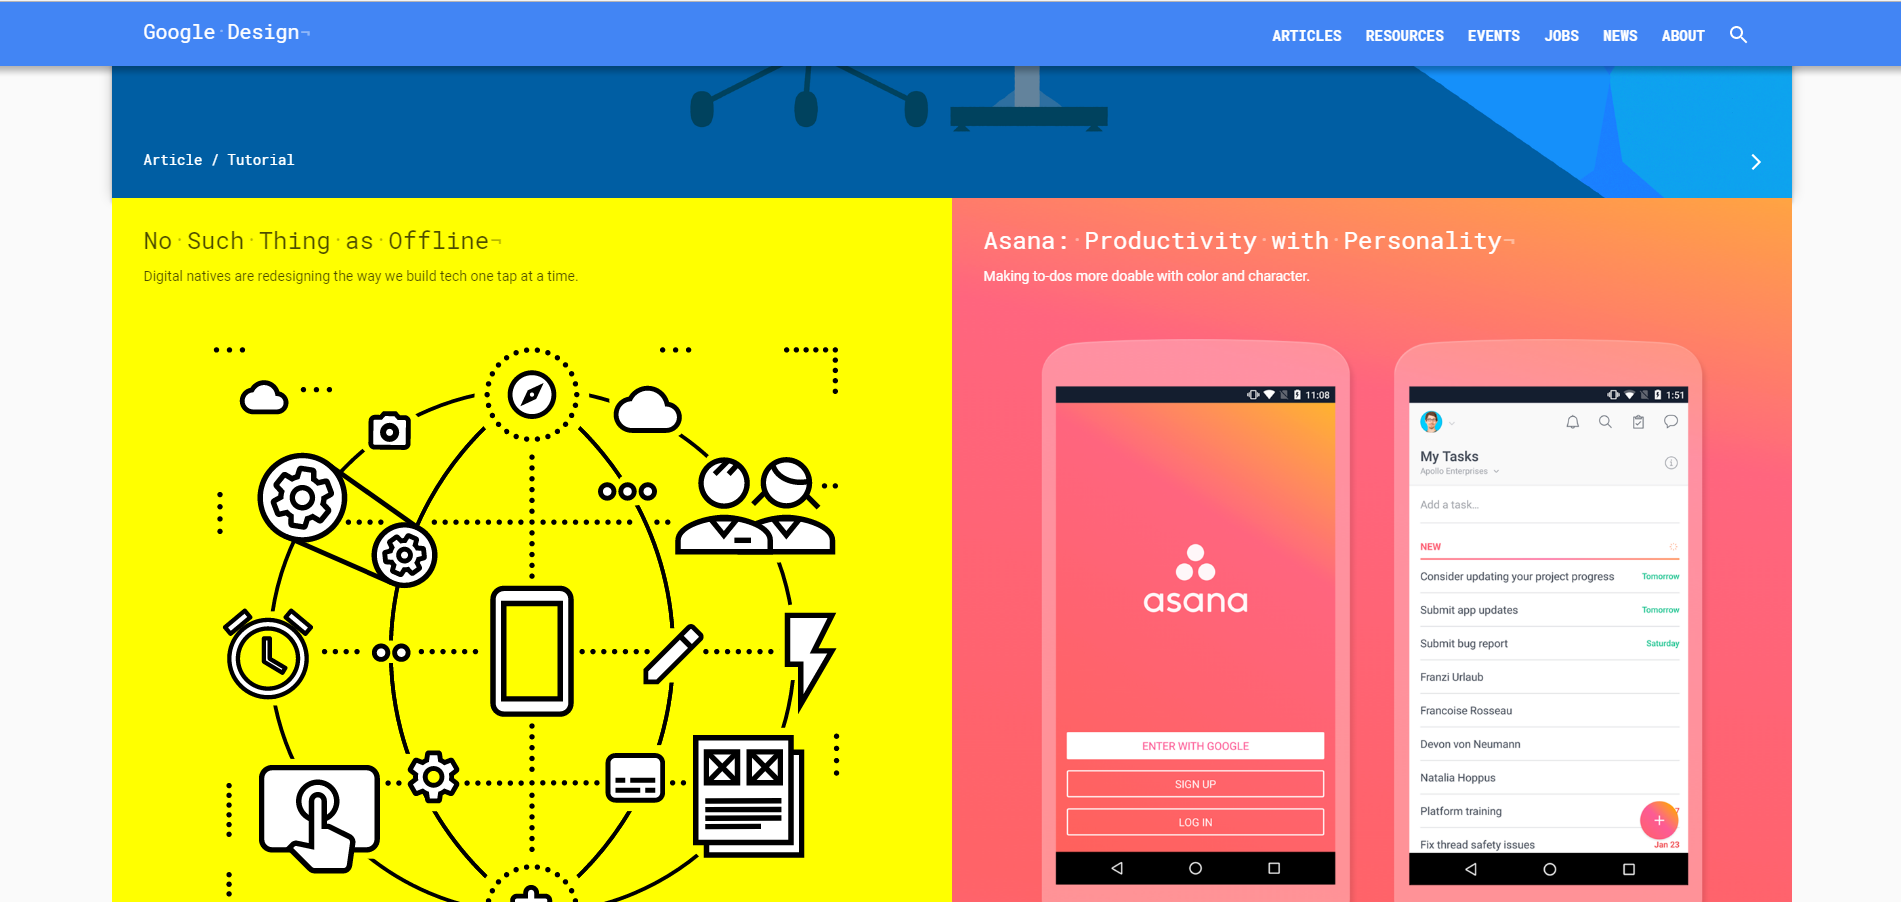
\includegraphics[max size={\textwidth}]{material}
\caption{Příklad tématu pro aplikaci napsanou technologií material.}
\label{material-fig}
\end{figure}

\paragraph{Boostrap} jeden z prvních responzivních rámců, který přivedl sjednocení uživatelského rozhraní napříč všemi platformami s největším důrazem na mobilní platformy. Dost často jsou vytvořeny webové aplikace, které nerespektují různé rozlišení pro různé uživatele, tomuto se chtěl bootstrap vyhnout. Nyní nabízí velké množství doplňků a rozšíření, díky kterým z něj dělají rázem nejrozšířenější responzivní rámec. \cite{bootstrap} Příklad aplikace napsané pomocí Bootstrapu můžeme vidět na oficiální tématu na \ref{bootstrap-fig}.

\begin{figure}[htp]
\centering
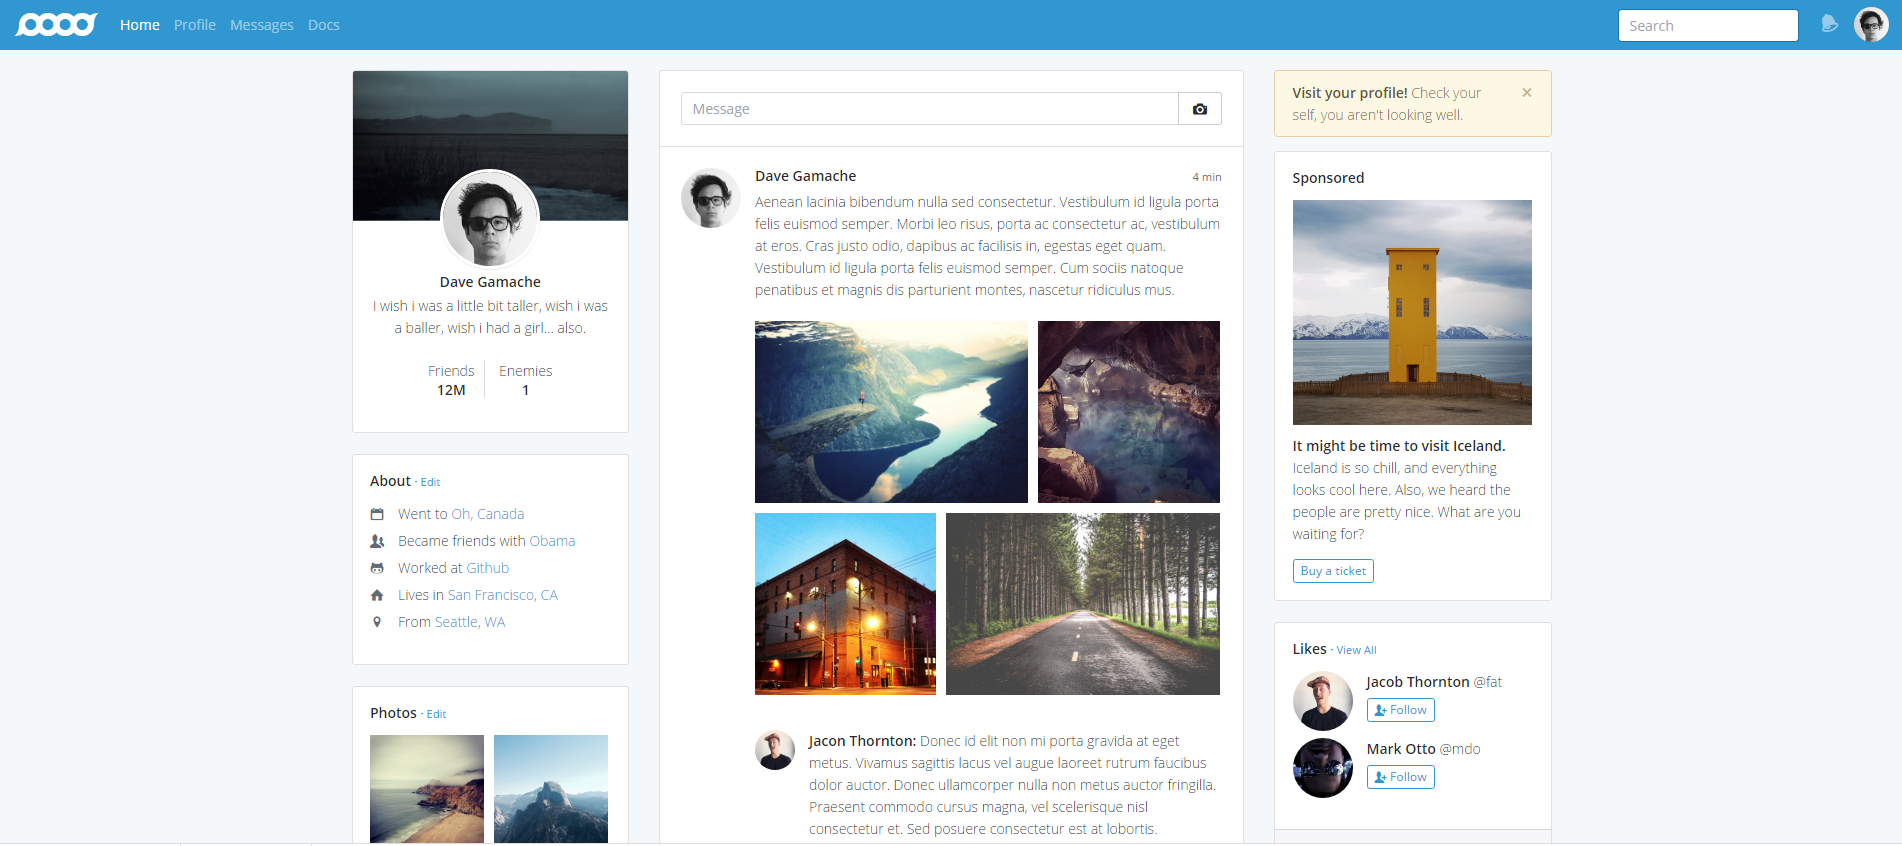
\includegraphics[max size={\textwidth}]{bootstrap}
\caption{Příklad tématu pro aplikaci napsanou technologií bootstrap.}
\label{bootstrap-fig}
\end{figure}

\paragraph{Patternfly} se inspiroval bootsrapem a vytvořil vlastní responzivní rámec, dále nabízí několik widgetů pro zobrazování složitějších uživatelských dat. Jeho hlavním zaměřením je unifikovat jednotlivé aplikace ve firmě, tak aby měli stejný, ale unikátní design. Proto nabízí několik jednoduchých přístupů co a jak dělat pro dosažení co nejvíce podobného vzhledu napříč aplikacemi. \cite{patternfly} Příklad aplikace napsané pomocí Materialu můžeme vidět na \ref{patternfly-fig}.

\begin{figure}[htp]
\centering
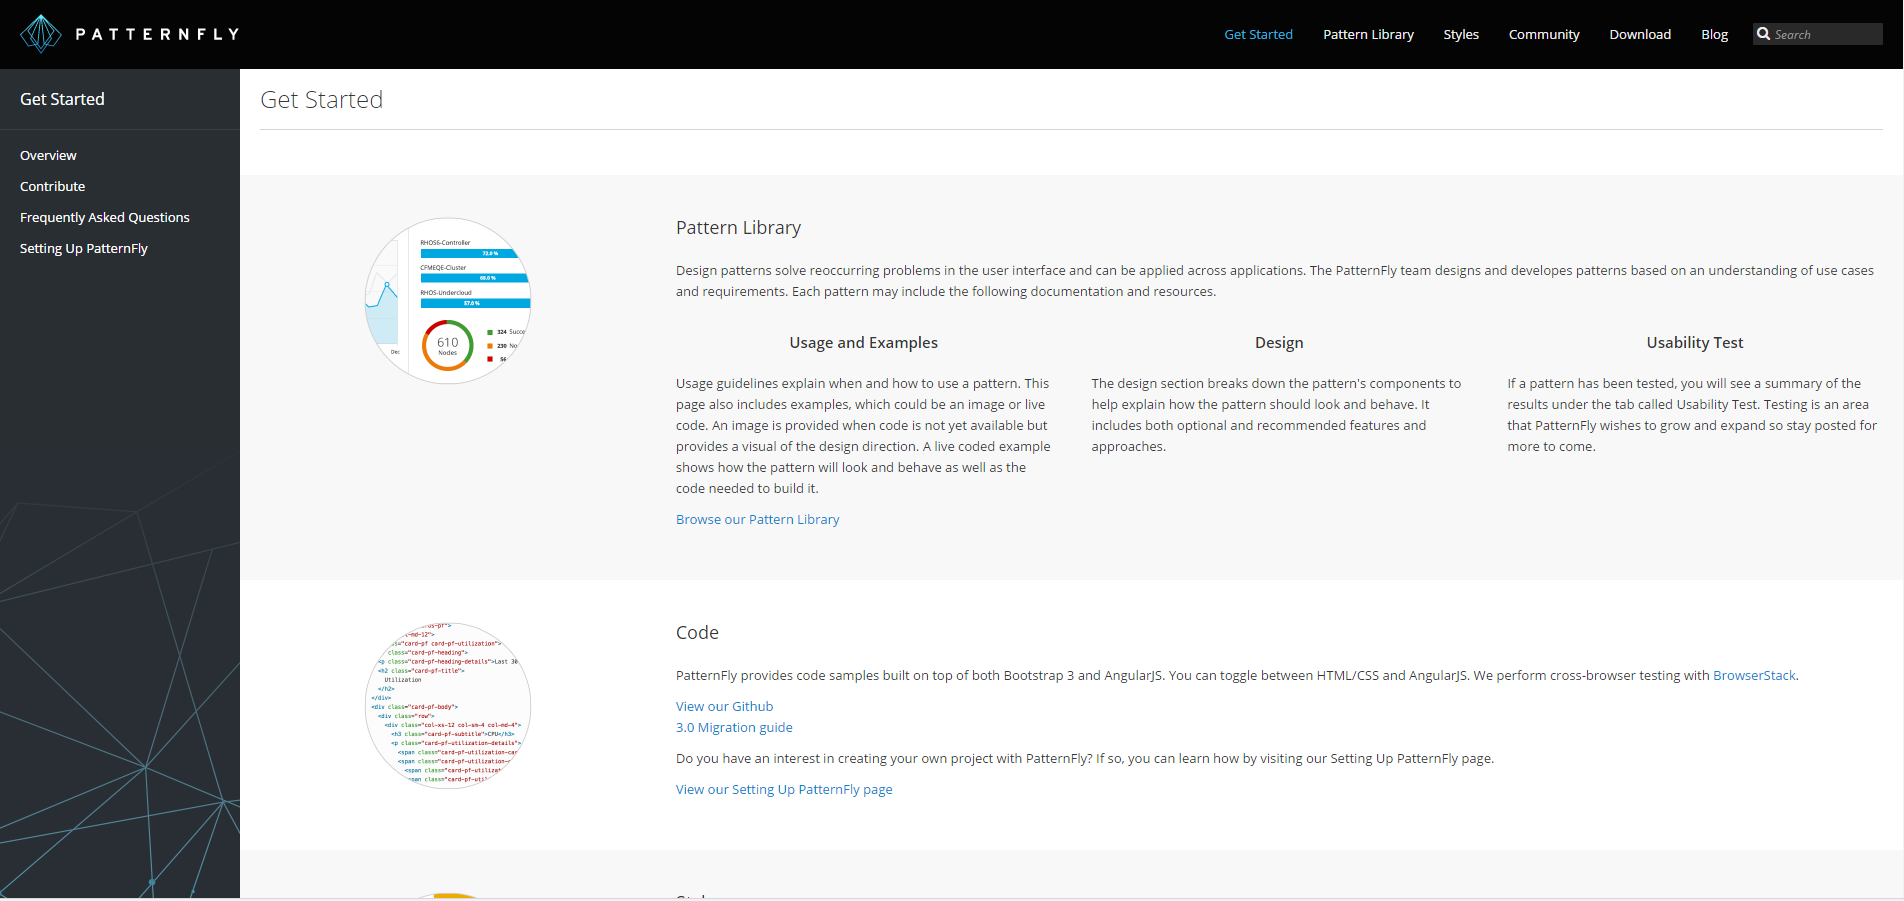
\includegraphics[max size={\textwidth}]{patternfly}
\caption{Příklad tématu pro aplikaci napsanou technologií patternfly.}
\label{patternfly-fig}
\end{figure}

\section{Single sign-on}
\par V aktuální době velká část společností nabízejících větší portfolio aplikací volí takzvanou službu single sign-on, kdy uživatel nemusí pokaždé zadávat své přihlašovací údaje, ale o jeho identifikaci se postará specializovaná služba. Většinou se stačí do této služby přihlásit jednou a dokud nevyprší čas od posledního použití aplikace, která používá tuto službu, nebo není uživatel schválně odhlášen nemusí se znovu přihlašovat. Jako protiklad je postaven Single sign-off, kdy při odhlášení v jedné aplikaci je uživatel automaticky odhlášen ze všech ostatních aplikací, toto napomáhá dalšímu zabezpečení.

\subsection{Standardy získání identity}
\par V aktuální době jsou pravděpodobně nejrozšířenější dva standardy použití SSO -- novější \textbf{OpenID Connect} a starší, ale robustnější \textbf{SAML}.
\paragraph{OpenID Connect} je v podstatě identifikační vrstva postavená nad OAuth 2.0, poskytuje možnost identifikace uživatele a také získání základních informací. Modernější a v aktuální době více používaný způsob převážně kvůli jeho jednoduchosti a nižšímu zatížení serveru. \cite{oidc}

\paragraph{SAML} se skládá ze dvou částí, poskytovatele služby a poskytovatele totožnosti (tím může být například Facebook, Google, Github, atd.). Jakým způsobem je uživatel přihlášen do služby můžeme vidět na obrázku \ref{saml2}. Nejdříve uživatel vytvoří požadavek na poskytovatele služby, ten vygeneruje SAML požadavek v URL, aplikace přesměruje uživatele na poskytovatele totožnosti, ten ověří přihlašovací údaje, přepošle zpět na poskytovatele služby požadavek na potvrzení, dále je uživatel přesměrován na cílový požadavake, o který si znovu požádá a server mu jej vrátí. \cite{saml}
\begin{figure}[!htp]
\centering
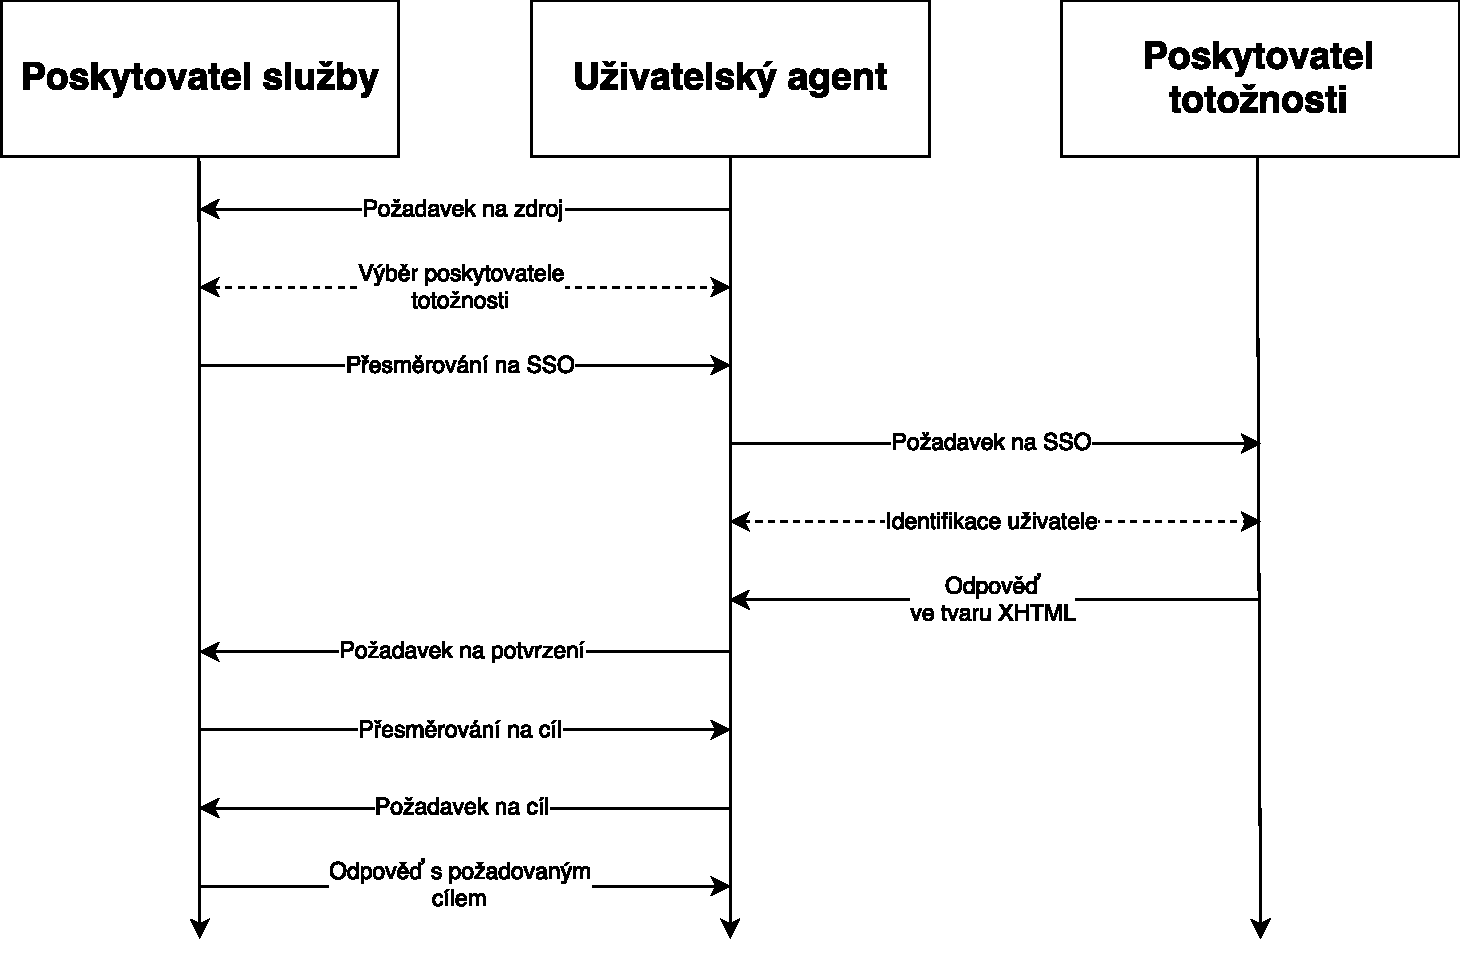
\includegraphics[max size={\textwidth}{\textheight}]{SAML2.pdf}
\caption{Předání uživatelského požadavku při použití SAML2}
\label{saml2}
\end{figure}

\subsection{Autentikační servery} \label{auth-server}
\par Aktuální trh nabízí velké množství autentizačních serverů, které spravují uživatele a poskytují přihlášení do více aplikací. Některé jsou dokonce volně k použití bez nutnosti zakoupit licenci, je nutné pouze spravovat servery na kterých takováto služba poběží. Mezi tyto servery patří například \textbf{Keycloak}, \textbf{Sterling externí autentizační server} a \textbf{Active Directory Federation Services}.

\paragraph{Keycloak} je open source řešení, které nabízí připojení jak přes sociální sítě a možnost získání uživatelských účtů z LDAP, Active Directory a nebo přímo z databáze. Jeho velkou premisou je jednoduchost správy uživatelů, včetně definice přístupových práv pro jednotlivé části aplikace. \cite{keycloak} Jak uživatel získá JWT při použití nástroje keycloak můžeme vidět na obrázku \ref{keycloak-jwt-fig}, kde si uživatel zažádá o nový token, kterým se poté autorizuje u aplikačního serveru.

\begin{figure}[htp]
\centering
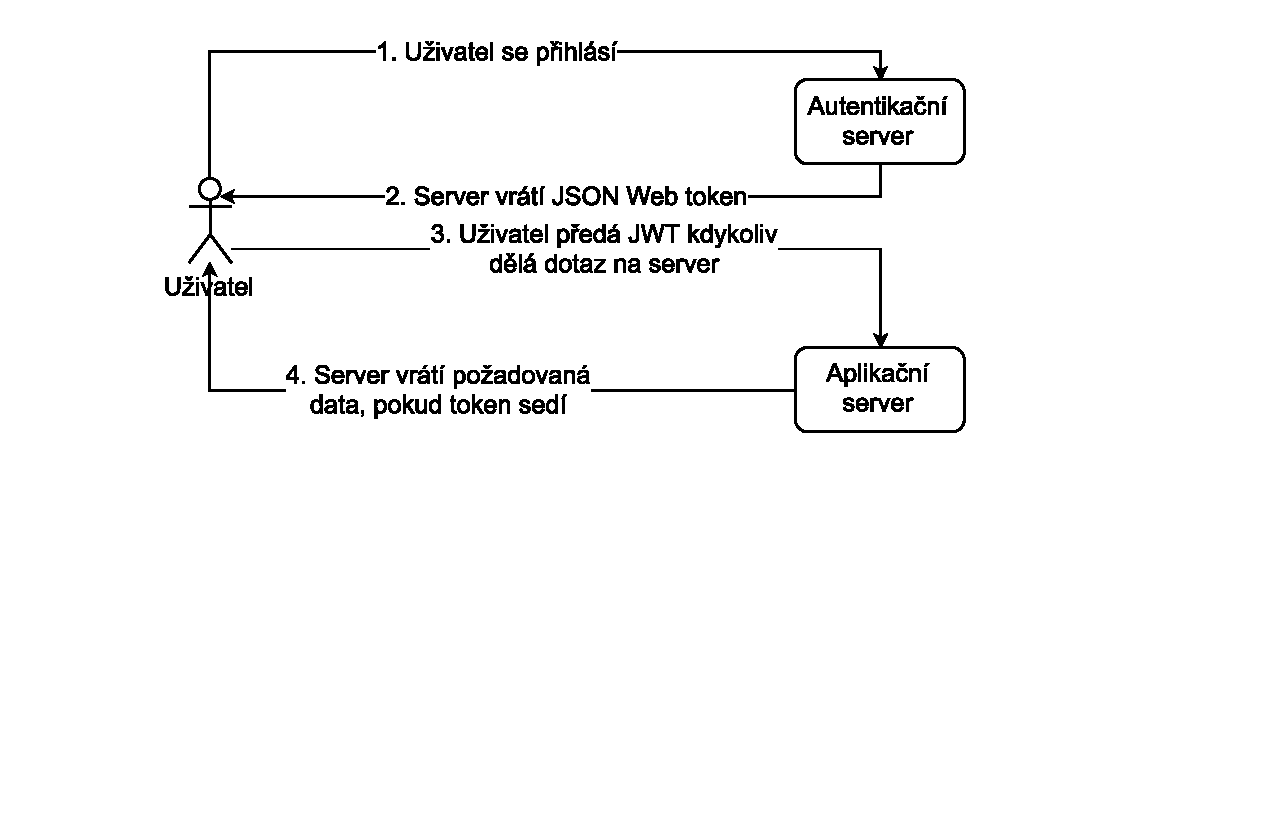
\includegraphics[max size={\textwidth}{\textheight}]{jwt.pdf}
\caption{Znázornění získání JWT z nástroje keycloak.}
\label{keycloak-jwt-fig}
\end{figure}

\paragraph{Sterling externí autentizační server} je řešení od IBM nabízející rozšířené autentizace a validace služeb pro IBM produkty, nabízí napojení například na LDAP a možnost SSH autentizace. \cite{ibm-ster}
\paragraph{Active Directory Federation Services} od firmy Microsoft nabízí možnost sdílet identifikační informace napříč důvěryhodným obchodním partnerům skrze extranet. Výhodou je že se nemusí aplikace starat o všechny uživatele, ale pouze si vyžádá od spřátelené aplikace jeho práva. \cite{ADFS}

\section{Datová analýza}
\par Pokud firma disponuje velkým množstvím dat je vhodné nad těmito daty najít nějaké souvislosti, které jí dopomůžou k vytváření dalšího zisku, případně pouze pro pochopení daného zákazníka, nebo skupiny zákazníků. Pokud je těchto dat opravdu hodně, můžeme je označit za Big Data (popsáno v \ref{big-data}), poté procesům k získání dalších informací říkáme Dolování dat (blíže popsáno v \ref{data-mining}).

\subsection{Shluková analýza}
\par Pro bližší pochopení velkého množství dat je vhodné použít metodu shlukoví analýzy, což je zjednodušené proces organizace objektů do skupin, tak aby její členové byli nějakým způsobem co nejvíce podobní. Shlukovou analýzu můžeme rozdělit do dvou skupin \textbf{nehierarchické} a \textbf{hierarchické}.

\paragraph{Nehierarchické} metody mohou být tvrdé nebo jemné, tvrdé seskupují data na základě specifické shlukové vlastnosti -- pokud patří do tohoto shluku namůže patřit do jiného. Jemné na druhou stranu nedefinují přesnou hranici -- patří do tohoto shluku, ale má některé vlastnosti datových bodů jiných shluků. Pro dělení můžeme použít metodu K-means, která přiřadí každý bod do shluku jemuž středu je nejblíže a při každém běhu algoritmu se středy shluků přepočítávají jako aritmetické průměry všech bodů.

\paragraph{Hierarchické} metody můžeme použít ve dvou způsobech ze shora dolů a odspodu nahoru. V prvním případě vezmeme všechny datové body a označíme jej za shluk, který poté rozdělíme na další shluky, které dále dělíme. Opět můžeme využít K-means pro dělení shluků. Druhý způsob (odspodu nahoru) je nejlépe použít v případě že máme menší vzorek dat a chceme co nejlepší shluk.

\par Pro shrnutí je potřeba si uvědomit dvě věci, jaký je nejmenší počet shluků a naopak jaký je největzší počet těchto shluků. Na první otázku je jednoduché odpovědět, je to v podstatě celý seznam datových bodů v jednom shluku (není nám to příliš užitečné, ale je to shluk dat). Na otázku největšího počtu shluků můžeme říct, že jím je počet všech datových bodů (toto opět není příliš užitečné). Proces shlukování je tedy rozdělování těchto dat do shluků větších jak jedna a menších než počet prvků, proces ukončíme v momentě, kdy jsme spokojeni s celkovým počtem shluků, případně velikostí těchto skupin.

\subsection{Rozhodovací stromy}
\par Tento algoritmus slouží k získání pravidel a vztahů v datovém souboru pomocí větvení. Díky použití stromů je tento algoritmus rychlý a výhodný pro použití s počítačem. Složení stromu je takové že na vrcholu je jeden uzel, kterému se říká kořen, ze kterého vede několik hran spojující vnitřní uzly, které mají opět několik hran promujících další uzly. Každý uzel musí mít právě jednoho předka (ne více ani méně), kromě kořenového uzlu, který nemá žádného předka. Výhodou je jednoduchost, efektivnost a možnost použít i pro velký objem dat, na druhou stranu pokud nám budou některá data chybět, nebo budeme mít spojitá data rozhodovací stromy budou mít problémy. Při výběru vlastnosti, která je nejvíce odlišná od ostatních příkladů v ostatních třídách se požívá takzvané entropie, její výpočet lze vidět na \ref{entropie}, kde \(p_t\) je pravděpodobnost výskytu třídy \(t\) a \(t\) je počet tříd
\begin{equation} \label{entropie}
E(S) = - \sum_{t=1}^{T}(p_t log_2 p_t)
\end{equation}

\par Pro vytvoření stromu se vezme tabulka hodnot a pro každý atribut se vypočítá jeho entropie, ta znázorňuje homogenitu prvku. Pokud je prvek naprosto homogenní (nacházející se ve všech atributech) jeho entropie je 0, naopak pokud je prvek naprosto heterogenní (nachází se pouze v jednom atributu) jeho entropie je 1. Při prvotním vytvoření rozhodovacího stromu je tedy potřeba mít co nejlepší trénovací data, nicméně velké množství dat může mít za následek příliš složitý strom, který je opět nepoužitelný (proto je potřeba dbát na vhodnou velikost učebních dat). Pokud nám vznikne složitý a ne příliš efektivní rozhodovací strom je vhodné použít takzvané prořezávání, kdy odstraníme nadbytečné podstromy (velice vhodné v případě že jsme použili velký vzorek dat pro vytvoření stromu).

\par Příklad algoritmu, který se používá pro vytváření rozhodovacích stromů je takzvaný ID3, je založen na booleovských hodnotách, používá hladové vyhledávání v prostoru \footnote{Pro bližší informace o hladovém prohledávání \url{http://www.how2examples.com/artificial-intelligence/tree-search}} a strom je vytvářen odshora dolů. Vstupní parametry tohoto algoritmu jsou \textbf{příklady} -- data na kterých je rozhodovací strom vytrénován \textbf{atributy} -- nad nimiž ude strom testován a \textbf{cílový atribut} -- tento atribut se bude vytvořený strom snažit predikovat. ID3 algoritmus byl několikrát vylepšen a upraven pro použití za různých podmínek jako například C4.5 (vhodné při chybějících, nebo spojitých datech), C5 (vylepšený C4.5), pro vytvoření binárních rozhodovacích stromů je například vhodné použít klasifikační a regresní stromy (CART), případně pro práci s opravdu velkým množstvím dat je možné použít algoritmus SPRINT.

\par Na obrázku \ref{decision-tree} můžeme vidět příklad stromu, který vznikl pro rozhodování zda jít hrát badminton, pro jeho vytvoření byl použit algoritmus ID3 s menším vzorekem dat.
\begin{figure}[htp]
\centering
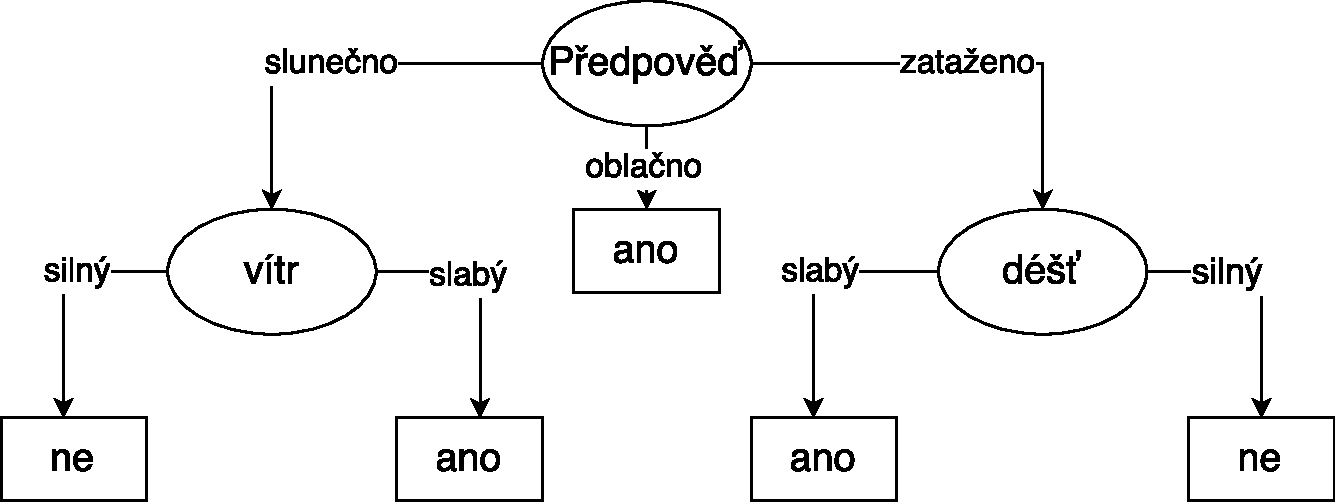
\includegraphics[max size={\textwidth}]{decision.pdf}
\caption{Příklad rozhodovacího stromu při použití algoritmu ID3.}
\label{decision-tree}
\end{figure}

\subsection{Dolování dat na webové aplikaci}
\par Toto získávání dalších informací z dat je v podstatě dolování z webových dokumentů, hyperlinků mezi nimi a získání informací z logů a webových stránek. \cite{minigbook}

\par Na webu lze využít několik možných technik dolování:
\begin{itemize}
\item \textbf{Webového obsahu} je proces získávání informací z webových dokumentů, mohou to být jak samotné stránky, tak videa, zvukových stop a obrázků. Hlavním zaměřením je však získání informací ze samotných textů na webovém dokumentu.
\item \textbf{Webové struktury} strukturu webových stránek si lze představit jako, uzlový graf, ve kterém jednotlivé uzly jsou samotné stránky a hrany spojující tyto stránky jsou vzájemné odkazy. Lze se také dále zanořit v jednotlivých dokumentech a ty znázornit pomocí stromové struktury \footnote{Přesný popis tohoto zápisu je znám pod zkratkou DOM (Document object model)}.
\item \textbf{Webového použití} je název pro označení technik, díky kterým lze získat další informace z používání webových stránek. Tyto data lze získat z několika zdrojů \textbf{webový server} -- záznamy, které vygeneroval server během jeho používání (IP adresy uživatelů, navštívenou stránku a čas navštívené stránky ...), \textbf{aplikační server} -- použití moderních aplikačních serverů dovoluje hladší vytvoření podnikových aplikací, tyto servery nadále dovolují bližší sledování uživatelských interakcí, \textbf{data aplikací} -- dále je možné v samotné aplikaci zapnout výpis dalších informací. \cite{minigbook}
\end{itemize}

\paragraph{PageRank} je označení pro stránkové ohodnocení, což má za následek vyšší skóre ve vyhledávacích nástrojích (jako je Google, Seznam, Yahoo, atd.). V jednoduchosti označují metriku pro ohodnocení dokumentů a zjištění jejich kvality. Takže hodnocení jednotlivých stránek záleží na hodnocení stránek, které odkazují na tuto stránku. Výpočet ohodnocení stránky \(p\) lze použitím rovnice \ref{pageRank}, kde \(n\) je počet odchozích uzlů, \(Outdegree(q)\) je počet hyperlinků na stránce q, \(d\) znamená pravděpodobnost, že uživatel zadá stránku přímo bez prokliknutí z jiné stránky a \(1 - d\) označuje pravděpodobnost že uživatel navštívá stránku z prokliknutého hyperlinku. \cite{minigbook}
\begin{equation} \label{pageRank}
PR(p) = d/n + (1-d) \sum_{(q,p) \in G}(\frac{PR(q)}{Outdegree(q)})
\end{equation}

\par Pro znázornění ohodnocení náhodné stránky se můžeme podívat na obrázek \ref{pageRankFig}, kde na jednu stránku ukazují tři stránky \textbf{P1}, \textbf{P2} a \textbf{P3}.
\begin{figure}[htp]
\centering
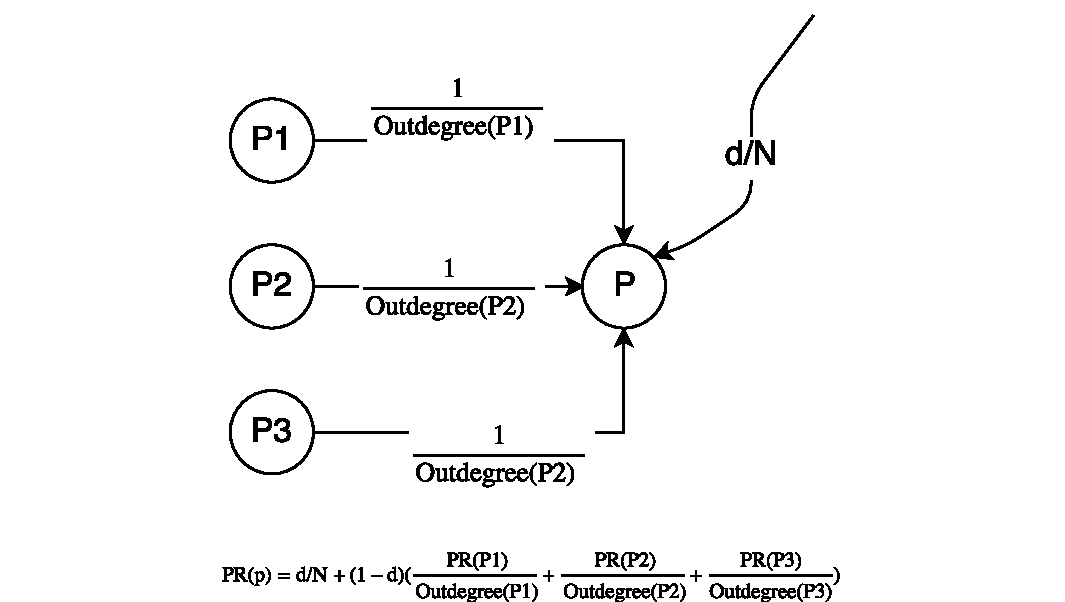
\includegraphics[max size={\textwidth}]{pagerank3.pdf}
\caption{Příklad hodnocení stránky pomocí Markovova modelu náhodné stránky.}
\label{pageRankFig}
\end{figure}

\subsection{Ukládání a práce s velkým objemem dat}
\par Při použití většiny technik na dolování dat je potřeba toto dolování spustit nad velkým množstvím dat, proto vzniklo několik technik jak na ukládání, tak na práci s tak velkým objemem dat. Pro ukládání se často příliš nehodí klasická relační databáze a proto se používají například takzvané NoSql databáze. Jednou z technik jak propojit několik datových uzlů je použít takzvané \textbf{Datové sklady} -- ty mají možnost připojit se na několik databází (bez ohledu na jejich typ) a za pomocí sofistikovaných reportingových nástrojů vytahovat z těchto databází informace, které dále transformují a upravují.

\par V případě použití NoSql databáze je potřeba data nějakým způsobem provázat (indexovat), aby s nimi šlo pracovat ve velice rychlém časovém úseku bez nutnosti při každém dotazu brát data přímo z databáze. Mezi indexovací nástroje patří například nástroje \textbf{Solr} \footnote{Jednoduchý a otevřený indexační nástroj \url{http://lucene.apache.org/solr/}} nebo \textbf{Elasticsearch} \footnote{Nástroj, který vyhledává a dokáže také analyzovat data \url{https://www.elastic.co/}}

\par Pokud naopak využijeme datových skladů můžeme pro následnou vizualizaci využít takzvané OLAP kostky, což je sada nástrojů pro práci s daty (mezi tyto nástroje patří například pivoting, řezy, drill down/up atd.)

\subsection{Aplikace využívající datovou analýzu}
\par V průběhu využívání dolování dat a využívání datové analýzy se nástroje a aplikace postupně zdokonalovali a začínají být čím dál tím více uživatelsky přístupné. Firmy se snaží propojit několik takovýchto aplikací a dát uživatelům silné nástroje pro snadné a rychlé získání dodatečných informací z velkého množství dat. Často se objevuje možnost připojit různé zdroje dat do těchto aplikací.

\paragraph{Power BI} je sada obchodních analytických nástrojů od firmy Microsoft, tyto nástroje vynikají především možností připojení na velké množství datových zdrojů a také možností publikovat vytvořené reporty na webové rozhraní takzvaný dashboard. Pro připojení na různé datové zdroje je použit nástroj Power BI gateway, který umožňuje, mimo jiné, připojit na rázné SQL databáze a analytické modely. \cite{powerbi}

\paragraph{IBM Watson Analytics} hlavní motto tohoto nástroje je poskytnutí silných a pokročilých analytických technik bez přílišné komplexnosti. Výhodou oproti ostatním nástrojům a aplikacím je jednoznačně možnost rychle, a bez nutnosti pokročilých technik dolování dat, získat ukryté informace v zákaznických datech. Tohoto docílí inženýři ve firmě IBM tím, že vyvinuli velice silnou a rychlou umělou inteligenci, která má za úkol hledat skrytou podstatu v datech. \footnote{Více o této umělé inteligenci pojmenované Watson se můžete dočíst zde \url{http://www.slate.com/blogs/future_tense/2014/02/14/watson_is_real_artificial_intelligence_despite_claims_to_the_contrary.html}} \cite{watson}

\paragraph{MicroStrategy} platforma podporuje dashboardy, interaktivní reporty a dotazování, upozornění a mnoho dalšího potřebného pro vytváření strategie podniku a zjišťování informací z dat. Tato platforma nevyužívá klasické multidimenzionální OLAP kostky, ale využívá relační OLAP architekturu, což umožňuje možnost použití nástroje drill down v jakékoliv dimenzi. Výhodou této platformy pro programátory je jistě dodávaný vývojářský balíček, který umožňuje dalšímu upravování vytvořených reportů a grafů. \cite{microstrategy}

\paragraph{SAP} nabízí hned dvě řešení pro možné dolování informací z dat \textbf{SAP BusinessObjects} a \textbf{SAP HANA}. První ze jmenovaných je sada fron-end aplikací která nabízejí uživateli prohlížet, řadit a pracovat s BI datami. Druhým je platforma, která má za úkol zpracovávat velké množství dat v reálném čase, jako bonus firma SAP nabízí vývojářský balík, kterým si uživatelé mohou upravit tuto platformu a rozšířit tak její využití. \cite{sap}

\section{Databázové aplikační platformy}
\par Mnoho firem v současné době nabízí různá řešení platforem, které zobrazují a umožňují práci s daty bez nutnosti instalace sofistikovaného programu u uživatele, ale za pomoci webového rozhraní. Tyto aplikace jsou převážně inspirovány úspěchem aplikace excel od firmy Microsoft, který v aktuální době používá více než 1,2 miliardy uživatelů \footnote{Podle oficiální zprávy od Microsoftu v roce 2016 \url{http://www.windowscentral.com/there-are-now-12-billion-office-users-60-million-office-365-commercial-customers}}. \par Firma Microsoft začala v nedávné době využívat možnost sdílet dokument mezi uživateli, kteří v reálném čase vidí změny prováděné na daném dokumentu. Podobnou funkci nabízí také firma Google, nicméně již nenabízí plnohodnotnou aplikaci, kterou by měl uživatel nainstalovanou na počítači a která by umožňovala uživateli pracovat pohodlněji s dokumenty (jak tomu je při použití aplikací od firmy Microsoft).

\paragraph{Fusioo} je webová aplikace, která nabízí jednoduchou integraci v rámci týmu pro správu důležitých informací. Je zde možné si nastavit dashboard, který nabízí metriky, grafy a upozornění. Jeho velkou výhodou je možnost provázanosti do kalendáře, díky které je možné jednoduše spravovat tým a jeho aktivity.

\paragraph{Ragic} tato platforma nabízí uživatelům možnost snadného přechodu z klasických excelových tabulek do databázového světa bez nutnosti jejich pochopení. Hlavním tahákem této platformy je určitě její chytré a intuitivní vyhledávání a při zadávání dat možnost zapnutí validace pro jednotlivé položky. Oproti konkurenci nabízejí neobvyklé reporty jako například TODO listy, nálepky, kontingenční tabulky a mapy.

\paragraph{Quickbase} je aplikace zaměřené na pokročilé uživatele, nenabízí příliš jednoduchý způsob zadání dat, nicméně dovoluje upravovat data v připojené databázi za pomoci nástroje, který připomíná Access od firmy Microsoft. Tato platforma se zaměřuje převážně na vývoj aplikací bez nutnosti psát kód, takovéto aplikace poté může zákazník dále nabízet ostatním uživatelům. Firma nabízí možnost definovat přístupová práva k jednotlivým dokumentům, skrze nastavení přístupových práv pro jednotlivé skupiny. Aplikace disponuje jedním velice zajímavým nástrojem grantovým diagramem, který napomáhá k rozvržení práce v rámci týmu a naplánování vývoje.

\paragraph{Knack} velice jednoduchá, nicméně snadno použitelná aplikace, která dovoluje uživatelům definovat databázi a následně ji spravovat oline pomocí webového rozhraní. V rámci definování dat je možné nastavit jejich strukturu -- určit jednotlivé typy pro záznamy, propojení -- jednotlivé záznamy mohou být navzájem propojené a získat tak další informace a uživatel také může definovat vzorce a formule. Nad konkurencí tento nástroj vede převážně díky možnosti snadno importovat a exportovat data.

\paragraph{Nintex workflow} platforma nabízí automatizaci procesů v rámci firmy, což znamená že zákazník může propojit jednotlivé aplikace (které jsou kompatibilní s aplikací Nintex) a systémy do určité posloupností úkolů, které dostanou zaměstnanci. Výhodou této platformy je především možnost propojení do velkého portfolia firemních aplikací, jako například NetSuite, Microsoft Dynamics a SAP, případně je možné vyvolat akci v podobě odeslání emailu, nebo SMS.

\section{Management vztahu se zákazníky (CRM)}
\par Je v podstatě termín používaný pro označení strategií a technologií použitých společnostmi pro monitorování a zjišťování stavu co uživatelé dělají s jejich produkty -- používají se jak k monitorování webových aplikací, tak volání, chatování, mailů a sociálních sítí. Mezi funkce CRM patří \textbf{automatizace marketingu}, \textbf{automatizace prodeje}, \textbf{automatizace kontaktního centra} a \textbf{geolokační technologie}. \cite{crm}

\begin{itemize}
\item \textbf{Automatizace marketingu} napomáhá marketingovému oddělení některé repetitivní úkoly provádět automaticky. Jako například při zavedení nového produktu není nutné psát každému zákazníku speciální email, ale nechat CRM systém vygenerovat speciálně cílenou reklamu pro každého zákazníka.
\item \textbf{Automatizace prodeje} eliminuje snahu prodat stejný produkt vícekrát různými zaměstnanci. Napomáhá ve sledování kdo a s jakou úspěšností se snaží daný produkt komu prodat.
\item \textbf{Automatizace kontaktního centra} usnadňuje komunikaci se zákazníky, dovoluje například nahrát zprávu, která se ozve všem zákazníkům s určitým problémem nebo dotazem (pokud se například problém nebo dotaz opakují).
\item \textbf{Geolokační technologie} některé CRM systémy dokonce disponují geolokační službu na základě které může podnik zjistit prodej určitého produktu napříč státy. \cite{crm}
\end{itemize}

\subsection{Monitorování webové aplikace}
\par V rámci zjišťování chování zákazníků na stránce může firma sáhnout po speciálním softwaru, který dovoluje jejich přesné monitorování. Díky tomuto monitorování může firma zjistit například v jakém kroku nákupu produktu zákazník odešel ze stránky a hlavně firma díky tomuto nástroji získá možnost přilákat nové zákazníky díky zjištění chování stávajících zákazníků. \cite{the-ux-book}

\paragraph{Google analytics} je poskytován zdarma od firmy Google, poskytuje statistické a základní nástroje analýzy používání webové stránky. Kromě toho, že je produkt zdarma má další výhody v podobě napojení na další nástroje od firmy Google, jako například \textbf{AdWords} \footnote{Placená služba, která dovoluje zákazníkům předplatit si reklamu na webových stránkách.}. Služba nabízí základní grafy a reporty spolu s možností zobrazit je na dashboardu. Těchto druhů dashboardu může být několik druhů -- základní, SEO analýza, sociální média, geografie, mobilní analýza, příchozí/odchozí a technický (uživatel si samozřejmě může vytvořit vlastní dashboard).

\paragraph{KissMetrics} je placená alternativa ke Google analytics, cílí především na velké webové stránky a nabízí mnoho způsobů jak monitorovat zákazníky. Mezi přední výhodu patří možnost identifikace uživatele ještě před jeho přihlášením, kdy se ukládá jeho pohyb do anonymního účtu a pokud se tento uživatel v budoucnu identifikuje všechna anonymní data se automaticky spárují s tímto účtem. Tento nástroj také nabízí mnohem jednodušší možnost nastavení A/B testování \footnote{A/B testování je v podstatě vytvoření dvou různých variant jedné stránky a testování, která je více úspěšnější mezi uživateli (více stráveného času, koupě produktu, více kliknutí na stránce ...)}, kdy není potřeba vytvořit dvě různé URL pro jednu stránku. Dále tento nástroj nabízí velice jednoduché nastavení sledování chování uživatelů na jednotlivých stránkách, kdy je velice snadné nastavit například sledování času stráveného na stránce, dobu vyplňování formuláře, pohyb kurzoru po stránce atd. Na obrázku \ref{ab-fig} můžeme lehce vidět výsledky A/B testování v nástroji KissMetrics.

\begin{figure}[htp]
\centering
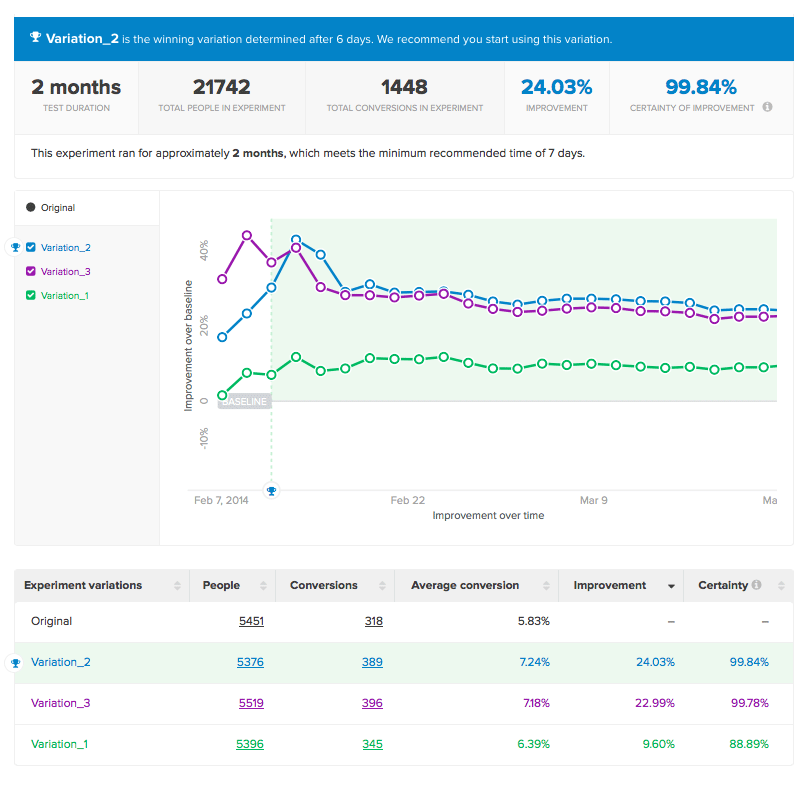
\includegraphics[max size={\textwidth}]{A_B}
\caption{Získání dat z A/B testování v nástroji KissMetrics.}
\label{ab-fig}
\end{figure}

\section{Shrnutí}
\par Aplikace zaměřující se na ukládání a práci s daty pomocí webového rozhraní se zaměřují převážně na větší podniky, případně nemají tolik intuitivní uživatelské rozhraní. Dále rozšiřitelnost dostupných aplikací není snadná a nastavení uživatelských práv je pouze v mizivém množství dostupných aplikací. Proto se dále zaměříme na vývoj samostatné aplikace, která spojí myšlenky z aktuálních aplikací a využije open source nástroje, které umožní snadnější práci s uživateli.

